% Options for packages loaded elsewhere
\PassOptionsToPackage{unicode}{hyperref}
\PassOptionsToPackage{hyphens}{url}
%
\documentclass[
]{book}
\usepackage{amsmath,amssymb}
\usepackage{lmodern}
\usepackage{setspace}
\usepackage{ifxetex,ifluatex}
\ifnum 0\ifxetex 1\fi\ifluatex 1\fi=0 % if pdftex
  \usepackage[T1]{fontenc}
  \usepackage[utf8]{inputenc}
  \usepackage{textcomp} % provide euro and other symbols
\else % if luatex or xetex
  \usepackage{unicode-math}
  \defaultfontfeatures{Scale=MatchLowercase}
  \defaultfontfeatures[\rmfamily]{Ligatures=TeX,Scale=1}
\fi
% Use upquote if available, for straight quotes in verbatim environments
\IfFileExists{upquote.sty}{\usepackage{upquote}}{}
\IfFileExists{microtype.sty}{% use microtype if available
  \usepackage[]{microtype}
  \UseMicrotypeSet[protrusion]{basicmath} % disable protrusion for tt fonts
}{}
\makeatletter
\@ifundefined{KOMAClassName}{% if non-KOMA class
  \IfFileExists{parskip.sty}{%
    \usepackage{parskip}
  }{% else
    \setlength{\parindent}{0pt}
    \setlength{\parskip}{6pt plus 2pt minus 1pt}}
}{% if KOMA class
  \KOMAoptions{parskip=half}}
\makeatother
\usepackage{xcolor}
\IfFileExists{xurl.sty}{\usepackage{xurl}}{} % add URL line breaks if available
\IfFileExists{bookmark.sty}{\usepackage{bookmark}}{\usepackage{hyperref}}
\hypersetup{
  pdftitle={Bayesian Models for Pest Detection},
  pdfauthor={Chris Malone},
  hidelinks,
  pdfcreator={LaTeX via pandoc}}
\urlstyle{same} % disable monospaced font for URLs
\usepackage{color}
\usepackage{fancyvrb}
\newcommand{\VerbBar}{|}
\newcommand{\VERB}{\Verb[commandchars=\\\{\}]}
\DefineVerbatimEnvironment{Highlighting}{Verbatim}{commandchars=\\\{\}}
% Add ',fontsize=\small' for more characters per line
\usepackage{framed}
\definecolor{shadecolor}{RGB}{248,248,248}
\newenvironment{Shaded}{\begin{snugshade}}{\end{snugshade}}
\newcommand{\AlertTok}[1]{\textcolor[rgb]{0.94,0.16,0.16}{#1}}
\newcommand{\AnnotationTok}[1]{\textcolor[rgb]{0.56,0.35,0.01}{\textbf{\textit{#1}}}}
\newcommand{\AttributeTok}[1]{\textcolor[rgb]{0.77,0.63,0.00}{#1}}
\newcommand{\BaseNTok}[1]{\textcolor[rgb]{0.00,0.00,0.81}{#1}}
\newcommand{\BuiltInTok}[1]{#1}
\newcommand{\CharTok}[1]{\textcolor[rgb]{0.31,0.60,0.02}{#1}}
\newcommand{\CommentTok}[1]{\textcolor[rgb]{0.56,0.35,0.01}{\textit{#1}}}
\newcommand{\CommentVarTok}[1]{\textcolor[rgb]{0.56,0.35,0.01}{\textbf{\textit{#1}}}}
\newcommand{\ConstantTok}[1]{\textcolor[rgb]{0.00,0.00,0.00}{#1}}
\newcommand{\ControlFlowTok}[1]{\textcolor[rgb]{0.13,0.29,0.53}{\textbf{#1}}}
\newcommand{\DataTypeTok}[1]{\textcolor[rgb]{0.13,0.29,0.53}{#1}}
\newcommand{\DecValTok}[1]{\textcolor[rgb]{0.00,0.00,0.81}{#1}}
\newcommand{\DocumentationTok}[1]{\textcolor[rgb]{0.56,0.35,0.01}{\textbf{\textit{#1}}}}
\newcommand{\ErrorTok}[1]{\textcolor[rgb]{0.64,0.00,0.00}{\textbf{#1}}}
\newcommand{\ExtensionTok}[1]{#1}
\newcommand{\FloatTok}[1]{\textcolor[rgb]{0.00,0.00,0.81}{#1}}
\newcommand{\FunctionTok}[1]{\textcolor[rgb]{0.00,0.00,0.00}{#1}}
\newcommand{\ImportTok}[1]{#1}
\newcommand{\InformationTok}[1]{\textcolor[rgb]{0.56,0.35,0.01}{\textbf{\textit{#1}}}}
\newcommand{\KeywordTok}[1]{\textcolor[rgb]{0.13,0.29,0.53}{\textbf{#1}}}
\newcommand{\NormalTok}[1]{#1}
\newcommand{\OperatorTok}[1]{\textcolor[rgb]{0.81,0.36,0.00}{\textbf{#1}}}
\newcommand{\OtherTok}[1]{\textcolor[rgb]{0.56,0.35,0.01}{#1}}
\newcommand{\PreprocessorTok}[1]{\textcolor[rgb]{0.56,0.35,0.01}{\textit{#1}}}
\newcommand{\RegionMarkerTok}[1]{#1}
\newcommand{\SpecialCharTok}[1]{\textcolor[rgb]{0.00,0.00,0.00}{#1}}
\newcommand{\SpecialStringTok}[1]{\textcolor[rgb]{0.31,0.60,0.02}{#1}}
\newcommand{\StringTok}[1]{\textcolor[rgb]{0.31,0.60,0.02}{#1}}
\newcommand{\VariableTok}[1]{\textcolor[rgb]{0.00,0.00,0.00}{#1}}
\newcommand{\VerbatimStringTok}[1]{\textcolor[rgb]{0.31,0.60,0.02}{#1}}
\newcommand{\WarningTok}[1]{\textcolor[rgb]{0.56,0.35,0.01}{\textbf{\textit{#1}}}}
\usepackage{longtable,booktabs,array}
\usepackage{calc} % for calculating minipage widths
% Correct order of tables after \paragraph or \subparagraph
\usepackage{etoolbox}
\makeatletter
\patchcmd\longtable{\par}{\if@noskipsec\mbox{}\fi\par}{}{}
\makeatother
% Allow footnotes in longtable head/foot
\IfFileExists{footnotehyper.sty}{\usepackage{footnotehyper}}{\usepackage{footnote}}
\makesavenoteenv{longtable}
\usepackage{graphicx}
\makeatletter
\def\maxwidth{\ifdim\Gin@nat@width>\linewidth\linewidth\else\Gin@nat@width\fi}
\def\maxheight{\ifdim\Gin@nat@height>\textheight\textheight\else\Gin@nat@height\fi}
\makeatother
% Scale images if necessary, so that they will not overflow the page
% margins by default, and it is still possible to overwrite the defaults
% using explicit options in \includegraphics[width, height, ...]{}
\setkeys{Gin}{width=\maxwidth,height=\maxheight,keepaspectratio}
% Set default figure placement to htbp
\makeatletter
\def\fps@figure{htbp}
\makeatother
\setlength{\emergencystretch}{3em} % prevent overfull lines
\providecommand{\tightlist}{%
  \setlength{\itemsep}{0pt}\setlength{\parskip}{0pt}}
\setcounter{secnumdepth}{5}
\usepackage{booktabs}
\usepackage{setspace}
\usepackage{amsmath}
\usepackage[algo2e,linesnumbered,ruled]{algorithm2e}
\usepackage{algorithm}
\ifluatex
  \usepackage{selnolig}  % disable illegal ligatures
\fi
\usepackage[]{natbib}
\bibliographystyle{plainnat}

\title{Bayesian Models for Pest Detection}
\author{Chris Malone}
\date{2022-05-01}

\begin{document}
\maketitle

\setstretch{1}
% Trigger ToC creation in LaTeX
\renewcommand{\baselinestretch}{1}\normalsize
\tableofcontents
\renewcommand{\baselinestretch}{2}\normalsize

\hypertarget{introduction}{%
\chapter{Introduction}\label{introduction}}

\hypertarget{lit-review}{%
\chapter{Literature review}\label{lit-review}}

\hypertarget{introduction-1}{%
\section{Introduction}\label{introduction-1}}

\begin{itemize}
\tightlist
\item
  Description of what this chapter is about
\item
  Outline of the chapter
\end{itemize}

\hypertarget{control-and-monitoring-of-tephritid-fruit-flies}{%
\section{Control and monitoring of Tephritid fruit flies}\label{control-and-monitoring-of-tephritid-fruit-flies}}

Costs associated with invasive and pest species can be varied and significant. Invasive species pose economic, social and environmental costs. Fruit flies are an example of an economically costly pest. Fruit flies lay eggs in ripening fruits and vegetables. Produce that has been infested with fruit fly larvae is not fit for sale, domestically or abroad. Further, even if produce has not been infested, local suppliers can charge a premium for supplying pest-free produce to international markets.

Governments have a responsibility monitor and eradicate potential biological invasions. In particular, the Australian government is bound by the Biosecurity act (??) to ensure a very low level of risk for animal and plant invasions. Effectively and efficiently controlling biological invasions requires a principled and rigorous approach to monitoring. However, monitoring biological species is difficult and costly. In particular, the cost of increasing monitoring intensity must be traded off against the cost of failing to detect an incipient invasion.

The manager's role is made more difficult when a pest population is \emph{subdetectable}. Populations may be subdetectable because they can persist at low rates; because they are \emph{taxonomically cryptic} (i.e.~hard to distinguish from well known native species); because they are \emph{behaviourally cryptic} (i.e.~behave in ways that help them avoid detection by predators; see \citet{kery2002}); or because the population is suppressed by efforts to eradicate them. Matters are made worse when tests to detect the presence of a population have extremely low sensitivity for other reasons. For example, monitoring traps for fruit flies have very low attractiveness. One study of Mediterannean fruit fly found that only 0.02\% of 38.8 million flies were recaptured after release, in a standard surveillance setup in Adelaide (\citet{ms2007}).

Suppose an outbreak of an invasive pest has occurred. Monitoring for the pest must then be intensified and localised to the area of suspicion. If the pest has since been eradicated, governments are incentivised to declare eradication quickly. This is because

On the other hand, if eradication has \emph{not} occured,

A necessary prerequisite for minimising the probability of failing to detect an existing invasion is to understand what can be inferred about the state of the population from what has been observed in surveillance. In particular, it is desirable to understand the likelihood that extinction has occurred, given that the species has not been detected over a certain period of time.

In Australia, Pest Free Area status is awarded to a number of . However, outbreaks of these pests are periodic. It is typical for PFA status to be suspended following an outbreak.

PFA status is economically valuable to producers in the relevant region. Firstly, there may be offshore markets which require that produce is supplied from a PFA for a given pest. Secondly, in some markets, PFA status may allow the supplier to receive a price premium for goods sold. In other words, PFA status increases the value of local produce on international markets.

\begin{itemize}
\tightlist
\item
  Current codes of practice suggest a lower catch rate required for an outbreak to be declared when supplementary traps are set, but probabilities have not been estimated rigorously.
\end{itemize}

As mentioned above, the manager seeks to minimise resources spent on surveillance, while minimising the chance that an eradication is declared when none has occurred. The general problem this thesis is concerned with is to infer whether or not an invasive species has been extinguished based on survey records.

\hypertarget{literature-background}{%
\section{Literature background}\label{literature-background}}

In this subsection, I will describe a number of models that have been applied to the problem of inferring species absence. Existing methods can be categorised as frequentist and Bayesian. The core difference between frequentist and Bayesian methods is in their treatment of the variables that describe the presence or absence of the species. Frequentist methods assume that the species is either absent or present with probability one. In this framework, surveillance activities are considered to be random experiments with fixed parameters. On the other hand, Bayesian methods assume that species absence is uncertain (i.e.~random).

\hypertarget{simple-models}{%
\subsection{Simple models}\label{simple-models}}

*** Note: Should I delete this entire subsection? I wrote it before I knew about the papers I discuss in the ``Elaborate models'' section.

\hypertarget{mcardle-1990}{%
\subsubsection{McArdle 1990}\label{mcardle-1990}}

I start by discussing the most basic approach to program design. This is the frequentist approach described by \citet{mcardle1990}. I emphasise this method because (a) it is conceptually simple and therefore easy to describe, and (b) it is emblematic of other methods in the literature, which are similarly general and simple. First, let the \emph{rarity} of the species \(p \in [0, 1]\) be the probability that a species is detected in any given sampling unit. (Sampling units can be arranged spatially or temporally; e.g.~a survey that involves checking \(w\) weeks at \(k\) locations would have \(wk\) sampling units.) Then, the number of surveys in which the species is detected is given by \(X \sim \mathrm{Binomial}(T, p)\). Accordingly, the probability of \emph{not} detecting the species in \(T\) surveys is given by
\[
\alpha = \Pr(X = 0) = 1 - (1 - p)^T.
\]

The last formula allows us to compute any of the 3 quantities \(\alpha\), \(p\), and \(t\), assuming the other two are given.

Given this framework, the problem of program design becomes the following. We decide \emph{a priori} what the smallest ``rarity'' \(p\) worth detecting is. McArdle supposes that if a species if sufficiently difficult to detect (while, nonetheless, \(p > 0\)) then it cannot be considered a member of an ecological community, and therefore not worthy of being deemed ``present''. Write the smallest rarity worth detecting as \(p_0\). Then, we choose a minimum detection probability \(\alpha\) that we are willing to accept. For example, we might wish to have chance \(\alpha > 0.95\) of detecting a species, given that it is present. Then, with the above formula, we can rearrange to get the smallest number of survey units \(T\) such that detection probability \(\alpha\) is achieved.

Statisticians will recognise that the above is essentially power analysis for data modelled as identically and independently distributed Bernoulli trials. This analogy can be made more concrete. For any fixed rarity \(p\), we can derive the probability of observing \(n\) or more negative surveys. This is the p-value. We can then reject the hypothesis that there is the rarity is greater than \(p_0\), the rarity worth detecting.

\hypertarget{limitations-of-mcardles-method}{%
\subsubsection{Limitations of McArdle's method}\label{limitations-of-mcardles-method}}

Applying the above model to the problem of program design is not straightforward. Firstly, the model is fairly restrictive. It assumes that the probability of detecting the pest population is constant over time. Secondly, in the case of pest populations, it may be difficult to determine the smallest value of \(p\) that is ``worth'' detecting. When a pest species is cryptic, the detectability (\(p\) in this model) can be extremely small even when the population is relatively large. Further, invasive potential of the pest may be large, so that even small populations bear a large cost to the decision maker.

\hypertarget{similar-models}{%
\subsubsection{Similar models}\label{similar-models}}

There are several other models in the literature, mirroring McArdle's method in their conceptual simplicity and generality. (See \citet{boakes2015} for a relatively complete review.) Bayesian models are given by \ldots{} and Barnes et al.~These methods have the advantage that the posterior distribution is derived analytically. This means that posterior probabilities can be computed extremely efficiently. However, each model assumes a constant growth rate. However, in real contexts, growth rates are highly variable and uncertain (\citet{caley2014}).

\hypertarget{elaborate-models}{%
\subsection{Elaborate models}\label{elaborate-models}}

\hypertarget{justification-for-elaborate-models}{%
\subsubsection{Justification for elaborate models}\label{justification-for-elaborate-models}}

Recently, more elaborate models have appeared in the literature for specific eradication inference problems. Here, I discuss the motivation and justification for these models.

\hypertarget{motivation}{%
\paragraph{Motivation}\label{motivation}}

As discussed above, simple models, such as McArdle's method, are attractive for their simplicity, generality, and efficiency of computation. However, these virtues may come at the cost of biological plausibility. This is particularly the case when we have a significant degree of prior information about the species and region in question. For high stakes problems, we would like to be able to leverage existing domain knowledge about the location and species. This might mean using process models that are fine grained, scientifically plausible, and based on multiple sources of scientific knowledge and evidence. We would also like to be able to incorporate our uncertainty about the processes in question.

List of problems to discuss\ldots{}

\begin{itemize}
\tightlist
\item
  They make strong assumptions about priors which are not defensible in general.

  \begin{itemize}
  \tightlist
  \item
    Assumption of a fixed, and either constant or declining population size (\citet{caley2015}, p.~2).
  \item
    For example, McArdle's model assumes that there is a value of \(p\) small enough to be not worth detecting.
  \end{itemize}
\item
  They assume that we can estimate a sighting rate, which is constant as a function of the locations of the individuals.
\end{itemize}

Another issue with simpler models is their relative inflexibility with respect to the structure of the model. For example, the method of Barnes et al assumes that we know the probability of detecting a specimen drawn randomly from the population. However, in the case of fruit flies, this number is difficult to estimate, because the capture probability is highly dependent on the trapping layout, which in turn is highly dependent on location and time. For example, countries (and states within countries) differ in the types of traps used and the spatial density of traps.

\hypertarget{plausibility}{%
\paragraph{Plausibility}\label{plausibility}}

As (\citet{caley2014}) points out, most models in the literature on the program design problem are simple and general. Their simplicity means that they are parsimonious, analytically tractable, and easy to interpret. However, these properties are bought at the cost of plausibility of the model as a description of real ecological processes, which are complex and uncertain. In general, the plausibility of a model will depend on the system that is under investigation. For a given model, the analyst may have information that will allow them to specify relatively more plausible and realistic models of the processes that govern the system.

\hypertarget{paper-1-keith-et-al}{%
\subsubsection{Paper 1: Keith et al}\label{paper-1-keith-et-al}}

The first instance of an elaborate Bayesian model for inferring pest eradication is given by \citet{keith2013}. The authors use an agent-based Bayesian model to infer the distribution of fire ant nests in Brisbane. They obtained data on the locations and month of discovery for \(n = 7{,}068\) nests. They also observed whether data were passively or actively discovered (e.g.~by members of the public or through a targeted search).

Generalised Gibbs sampling is used to sample\ldots{}

\hypertarget{sampling}{%
\subsubsection{Sampling}\label{sampling}}

It should be noted that both of the models above are agent based. The model of Keith et al explicitly models the location of each agent (ant nest). In each case, this leads to a difficulty in sampling algorithms. Typically, when a Bayesian model is agent based, this means that there is an unknown number of parameters in the model (and unbounded, as the size of the population typically does not have a finite bound, e.g.~when it is Poisson distributed). The upshot of this is that typical Markov Chain Monte Carlo (MCMC) methods, such as the Metropolis Hastings sampler, fail. This is because they do not allow us the dimension of the parameter vector to vary between draws.

The papers discussed above deal with this in two different ways. Keith et al use a generalisation of the Gibbs sampler, inspired by reversible jump MCMC. This gets around the problem by adding a step to the Gibbs sampler in which we move between coordinate spaces . On the other hand, Caley et al use approximate Bayesian computation (ABC).

\hypertarget{paper-2-caley-et-al}{%
\subsubsection{Paper 2: Caley et al}\label{paper-2-caley-et-al}}

The second instance of an elaborate Bayesian model for inferring eradication is given by \citet{caley2015}. Caley and co-authors develop a Bayesian model of fox sightings in Tasmania. Their goal is to infer the posterior probability that foxes had been eradicated in Tasmania, given a record of fox carcass sightings. They obtained data on fox carcass sightings from hunter kills and road kills. These observation processes were modelled separately, so that posterior detection rates differed between the sighting types. Detection rates were assumed to be constant across time and location for each type of sighting. Notably, uninformative priors were set for detection rates (i.e.~the probability of detecting a fox was set to be uniform on \([0, 1]\)). Data consisted of a single sighting count for each location (with Tasmania divided geographically into grid cells) and each year between 2001 and 2013. Data were all zeroes with the exception of exactly four unit observations (sightings of exactly one fox).

The authors use a simple rejection algorithm to sample from the posterior. I will refer to this algorithm as exact Bayesian computation (EBC), to be distinguished from approximate Bayesian computation (ABC). ABC works by first drawing samples of the parameter vector \(\theta\) from the prior distribution \(\pi(\theta)\), then second, drawing simulated data \(y_{\text{sim}}\) from the likelihood, then keeping the proposed \(\theta\) if and only if \(y_{\text{sim}}\) is an approximate match with the observed data. EBC is the same, except that samples are only kept if \(y_{\text{sim}}\) is an \emph{exact} match with the observed data. Notably, EBC is only practical in cases where the data consists entirely of discrete variables (i.e.~variables with countable or finite ranges of possible values).

The authors point to the complexity of the likelihood to justify the use of ABC over more standard Monte Carlo methods such as Metropolis Hastings or Gibbs sampling. Based on their description of the model, however, it is not clear that Metropolis Hastings would not suffice.

\hypertarget{gaps}{%
\section{Gaps}\label{gaps}}

Above, I have discussed the two elaborate computational models in the literature for inferring eradication of an incipient biological invasion. The current work seeks to address two gaps in the literature. Firstly, elaborate Bayesian models have not been explored for inferring eradication of Tephritid fruit flies. Fruit flies pose an interesting case study, because the regulator has fine grained information about the detection system. In particular, the regulator knows the locations of each of the traps. Further, prior research investigating the efficacy of these traps exists. If used carefully, this information can be leveraged through the model's priors to learn from the zero-sighting record efficiently.

Fruit flies are interesting for a few reasons:

\begin{itemize}
\tightlist
\item
  A body of research exists to understand trap efficacy.
\item
  The surveillance program is predictably structured
\item
  The intensity of the surveillance program changes in a predictable way.
\end{itemize}

Second, no such model has addressed the question of PFA status reinstatement. Instead, they discuss inferring eradication from an actually observed record.

\hypertarget{case-study-ceratatis-capitata}{%
\chapter{Case study: Ceratatis capitata}\label{case-study-ceratatis-capitata}}

\hypertarget{introduction-2}{%
\section{Introduction}\label{introduction-2}}

\hypertarget{what-this-chapter-is-about}{%
\subsection{What this chapter is about}\label{what-this-chapter-is-about}}

In the previous chapter, I proposed to address a gap in the literature by providing an elaborate model for inferring the eradication of an incipient invasive population of Tephritid fruit flies. In this chapter, I develop and present such a model.

\begin{itemize}
\tightlist
\item
  Note that this analysis is primarily illustrative. Performing a more specific analysis requires access to confidential data.
\item
  Note that the method can be used for a real scenario - we only need to change the priors, data and locations of the traps.
\item
  Note that I use a simplified model of Medfly dynamics for illustrative purposes - but the method can easily incorporate more complex ABS models, and cite those models.
\end{itemize}

\hypertarget{outline-of-this-chapter}{%
\subsection{Outline of this chapter}\label{outline-of-this-chapter}}

In this chapter, I present an illustrative model of medfly surveillance after an hypothetical invasion. I use a simplified model of Medfly population dynamics. However, for various species of Tephritid fruit fly (medfly included) detailed models exist. A benefit of the proposed method is that it can easily incorporate almost any model of medfly dynamics.\footnote{Note, though, that the sampling method I use may not be appropriate in all cases. When the model predicts that the population size ``explodes'', then the rejection rate for the sampling algorithm may become very high, causing the algorithm to be highly inefficient.}

\hypertarget{background}{%
\section{Background}\label{background}}

\hypertarget{medfly-are-economically-important}{%
\subsection{Medfly are economically important}\label{medfly-are-economically-important}}

Mediterranean fruit fly (\emph{Ceratitis Capitata}) or \emph{medfly} is a fly species native to sub-Saharan Africa. It is considered to be of high economic importance, due to its potential for destruction of fruit production (\citet{sciarretta2018}). Medfly has high invasive potential, as it can adapt to a relatively large range of climates and environments, and is known to have the capability to infest the fruits of over 300 species of plants (Ibid.).

\hypertarget{medfly-are-cryptic}{%
\subsection{Medfly are cryptic}\label{medfly-are-cryptic}}

Medfly are very hard to detect at low levels. Monitoring for medfly is typically performed with the aid of lured traps (namely so-called Lynfield or Jackson traps). These traps are relatively ineffective for detecting medfly. For example, one study from the Adelaide metro area trapping grid found that only 0.02\% of flies were recaptured from a release of 38.8 million flies. Further, medfly are known to have low dispersals across space. This means that low-lying populatons of flies may go undetected across generations. \url{https://onlinelibrary-wiley-com.virtual.anu.edu.au/doi/pdfdirect/10.1111/j.1570-7458.2006.00415.x}

\hypertarget{data}{%
\section{Data}\label{data}}

\hypertarget{zero-sighting-surveillance-data}{%
\subsection{Zero sighting surveillance data}\label{zero-sighting-surveillance-data}}

In this section, I do not use real data to estimate parameters. Instead, I model a hypothetical situation in which we observe \(\mathbf y = \mathbf 0_T\) (see above). The situation is as follows: We assume that at least one fly has been detected; eradication measures have since begun and then ceased; and we now proceed with intensified monitoring, while whatever population that may exist is free to grow relatively unhindered. By intensified monitoring, I mean that \textbf{supplementary} monitoring traps have been placed alongside the previously existing grid of \textbf{general} monitoring traps. More precisely, it is assumed that \textbf{general} exist year round in a 400 \(\times\) 400 metre grid (DPIPWE, 2011, p.~50). The \textbf{supplementary} surveillance system consists of a set of 16 traps in a circular area, centred at the site of the first fly detection.\footnote{It is typical to wait until at least 2 flies have been detected near each other for an outbreak to be declared. To illustrate the method in a simplified setting, I suppose that one fly detection is sufficient.} The goal of the analysis is to infer the probability of eradication for the incipient population, given no flies detected at any point in this period.

The data is a hypothetical survey record. We assume a fairly realistic scenario. We observe the outcomes of a surveillance process. The surveillance process is generated by weekly checks of traps that are deployed uniformly in a given area (more about the trapping arrangement below). It is assumed that no specimens are detected at any point in the survey period. In other words, the sum of all detected counts in the period is zero.

\hypertarget{data-on-capture-probability}{%
\subsection{Data on capture probability}\label{data-on-capture-probability}}

Above, I described the ``data'' under the model. This is the set of variables that we condition on to infer the posterior distribution. However, we can use data from other sources to inform our prior distribution over the model's parameters.

In cases where Bayesian models have been used, data has not been available on detection rates. For example, \citet{caley2014} and \citet{keith2013} set uninformative priors on the detection rates, and attempt to learn the detection rates for data. In the case of medfly, however, there is a body of experimental literature which can be used to understand capture rates for the species.

\hypertarget{model}{%
\section{Model}\label{model}}

In this section, I discuss a model of medfly dynamics and detection.

\hypertarget{full-model-overview}{%
\subsection{Full model overview}\label{full-model-overview}}

I break the model into the following three components: (1) The size of the population (number of individuals); (2) the locations of individuals and traps; and (3) number of individuals caught in traps, conditional on (1) and (2).

The likelihood of a given number of captures is a function of latent variables, namely the number and locations of flies. Under the prior distribution, it is assumed that data at any given timestep are generated as follows. Firstly, nature draws a number of flies (i.e.~a population size) which may or may not be based on the number of flies at the previous time step. Next, nature draws a location for each of the flies. Finally, nature draws a number of detections.

\hypertarget{the-population-size}{%
\subsection{The population size}\label{the-population-size}}

The growth model describes our prior beliefs about how a population of size \(N_1\) might grow or decline over time.

\begin{itemize}
\tightlist
\item
  Overview
\item
  Technical details
\item
  Specific priors
\end{itemize}

\hypertarget{overview}{%
\subsubsection{Overview}\label{overview}}

A natural way to set a prior on the population size at each time point \(t\) is to set a prior on the population size at the initial time point, and then assume that the population sizes at other time points are given by some (deterministic or stochastic) function of the population size at \(t-1\), and the value of a covariate vector \(X_t\), which includes variables relevant to population growth.

It may be worth noting that there are no a priori assumptions on the population dynamics for the growth model. Thanks to the generality of the sampling algorithm, it is simple to ``plug in'' elaborate growth models. For example, the models of \citet{lux2018} or \citet{manoukis2014} could be used to generate independent random draws from the population of Medfly. In this way, they can structure our prior over the population size. In this case, inference would proceed simple as in the case I outline here. This highlights a benefit of the modelling approach taken here, which is its generality and modularity.

\[
N_t = f(N_{t-1}, X_t)
\]

\hypertarget{technical-details}{%
\subsubsection{Technical details}\label{technical-details}}

As for prior distributions on \(N_t\), for \(t \in \{1, \ldots, T\}\), a growth model is used to structure the prior. Namely, an exponential growth model is assumed, so that \(N_t = \mathrm{round}[N_{t-1} \exp\{R_t\}]\), where \(R_t\) is the growth rate at time \(t\). The exponential growth model is chosen for its ubiquity in ecological science in general, and in studies of fruit fly dynamics in particular. Rounding is introduced to give \(N_t\) discrete support. The growth parameter \(R_t\) is uncertain, and based on temperature.\footnote{Alternatively, we could leave the rounding step out, and interpret \(N_t\) as the expected number of flies at each step. I do not consider this possibility in any further depth.}

\hypertarget{popoulation-size-priors}{%
\subsubsection{Popoulation size priors}\label{popoulation-size-priors}}

In this case, \(N_1\) is the first week after the most recent fly detection. I have chosen to give \(N_1\) the prior distribution \(N_1 \mid \lambda \sim \mathrm{Poisson}(\lambda)\), where \(\lambda \sim \mathrm{Exponential}(\gamma)\). I have set \(\gamma\) to \(0.05\). This distribution for \(N_1\) is chosen as it is a discrete distribution with right skew, and a relatively large amount of mass \(f_{N_1}(x)\) at \(x = 0\), corresponding to the situation where flies are already eradicated.

\begin{Shaded}
\begin{Highlighting}[]
\NormalTok{g }\OtherTok{=} \DecValTok{1}\SpecialCharTok{/}\DecValTok{20}
\NormalTok{init\_pmf }\OtherTok{=} \ControlFlowTok{function}\NormalTok{(n, g) g }\SpecialCharTok{/}\NormalTok{ (}\DecValTok{1}\SpecialCharTok{+}\NormalTok{g)}\SpecialCharTok{\^{}}\NormalTok{(n}\SpecialCharTok{+}\DecValTok{1}\NormalTok{)}

\NormalTok{x }\OtherTok{=} \DecValTok{0}\SpecialCharTok{:}\DecValTok{100}

\NormalTok{df }\OtherTok{=} \FunctionTok{data.frame}\NormalTok{(}\AttributeTok{x =}\NormalTok{ x, }\AttributeTok{y =} \FunctionTok{init\_pmf}\NormalTok{(x, g))}

\FunctionTok{ggplot}\NormalTok{(df) }\SpecialCharTok{+}
  \FunctionTok{geom\_bar}\NormalTok{(}\AttributeTok{stat =} \StringTok{\textquotesingle{}identity\textquotesingle{}}\NormalTok{, }\FunctionTok{aes}\NormalTok{(x, y)) }\SpecialCharTok{+}
  \FunctionTok{xlab}\NormalTok{(}\FunctionTok{bquote}\NormalTok{(}\FunctionTok{italic}\NormalTok{(n))) }\SpecialCharTok{+}
  \FunctionTok{ylab}\NormalTok{(}\FunctionTok{bquote}\NormalTok{(}\StringTok{\textquotesingle{}Pr(\textquotesingle{}}\SpecialCharTok{*}\FunctionTok{italic}\NormalTok{(N)[}\DecValTok{1}\NormalTok{] }\SpecialCharTok{==} \FunctionTok{italic}\NormalTok{(n)}\SpecialCharTok{*}\StringTok{\textquotesingle{})\textquotesingle{}}\NormalTok{))}
\end{Highlighting}
\end{Shaded}

\begin{figure}
\centering
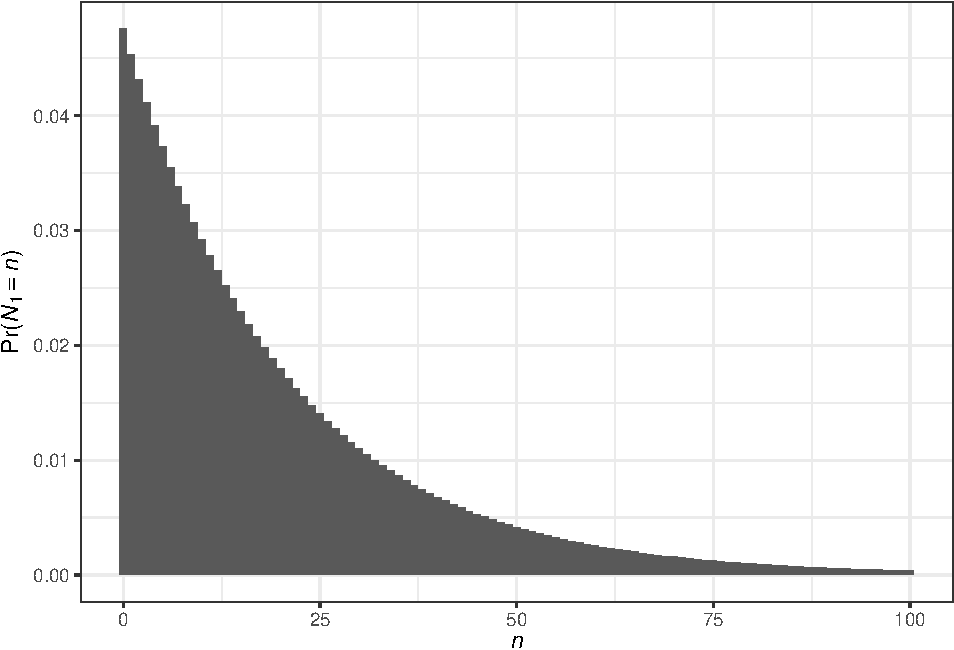
\includegraphics{_main_files/figure-latex/prior_init_size-1.pdf}
\caption{(\#fig:prior\_init\_size-1)Prior distribution of initial population size}
\end{figure}

\begin{Shaded}
\begin{Highlighting}[]
\CommentTok{\# Prior probability that they\textquotesingle{}re already eradicated}
\FunctionTok{curve}\NormalTok{(}\FunctionTok{exp}\NormalTok{(g}\SpecialCharTok{\^{}}\DecValTok{2} \SpecialCharTok{*}\NormalTok{ x}\SpecialCharTok{\^{}}\NormalTok{(g}\DecValTok{{-}1}\NormalTok{)))}
\end{Highlighting}
\end{Shaded}

\begin{figure}
\centering
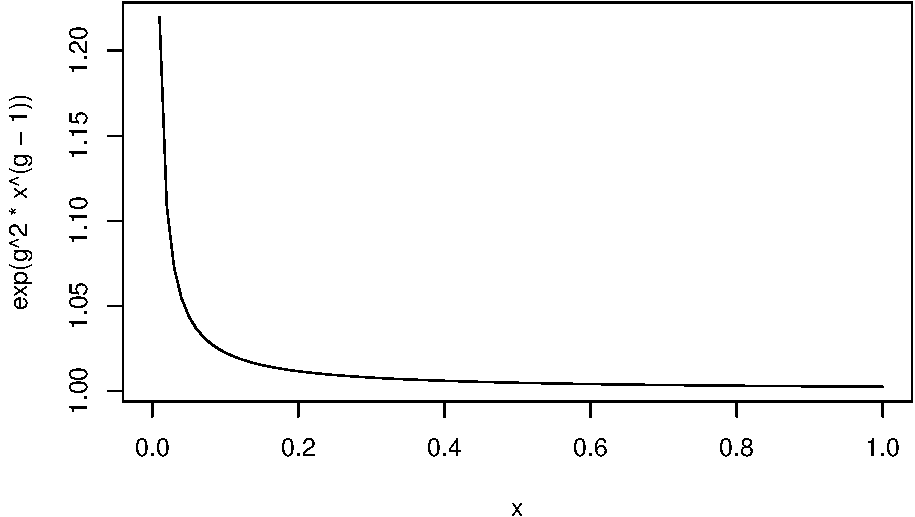
\includegraphics{_main_files/figure-latex/prior_init_size-2.pdf}
\caption{(\#fig:prior\_init\_size-2)Prior distribution of initial population size}
\end{figure}

\begin{Shaded}
\begin{Highlighting}[]
\NormalTok{prior\_prob }\OtherTok{=} \ControlFlowTok{function}\NormalTok{(x) g}\SpecialCharTok{\^{}}\DecValTok{2} \SpecialCharTok{*}\NormalTok{ x}\SpecialCharTok{\^{}}\NormalTok{(g}\DecValTok{{-}1}\NormalTok{)}

\NormalTok{x }\OtherTok{=} \FunctionTok{seq}\NormalTok{(}\DecValTok{0}\NormalTok{, }\DecValTok{1}\NormalTok{, }\FloatTok{0.001}\NormalTok{)}

\NormalTok{df\_dens }\OtherTok{=} \FunctionTok{data.frame}\NormalTok{(}\AttributeTok{x =}\NormalTok{ x, }\AttributeTok{y =} \FunctionTok{prior\_prob}\NormalTok{(x))}
\FunctionTok{ggplot}\NormalTok{(df\_dens) }\SpecialCharTok{+}
  \FunctionTok{geom\_function}\NormalTok{(}\AttributeTok{fun =}\NormalTok{ \textbackslash{}(x) g }\SpecialCharTok{*}\NormalTok{ x}\SpecialCharTok{\^{}}\NormalTok{(g}\DecValTok{{-}1}\NormalTok{), }
                \AttributeTok{n =} \FloatTok{1e4}\NormalTok{) }\SpecialCharTok{+}
  \FunctionTok{xlim}\NormalTok{(}\FunctionTok{c}\NormalTok{(}\DecValTok{0}\NormalTok{, }\FloatTok{0.01}\NormalTok{)) }\SpecialCharTok{+}
  \FunctionTok{ggtitle}\NormalTok{(}\StringTok{\textquotesingle{}Density of initial (prior) probability of eradication\textquotesingle{}}\NormalTok{) }\SpecialCharTok{+}
  \FunctionTok{xlab}\NormalTok{(}\StringTok{\textquotesingle{}x\textquotesingle{}}\NormalTok{) }\SpecialCharTok{+}
  \FunctionTok{ylab}\NormalTok{(}\StringTok{\textquotesingle{}Density\textquotesingle{}}\NormalTok{)}
\end{Highlighting}
\end{Shaded}

\begin{figure}
\centering
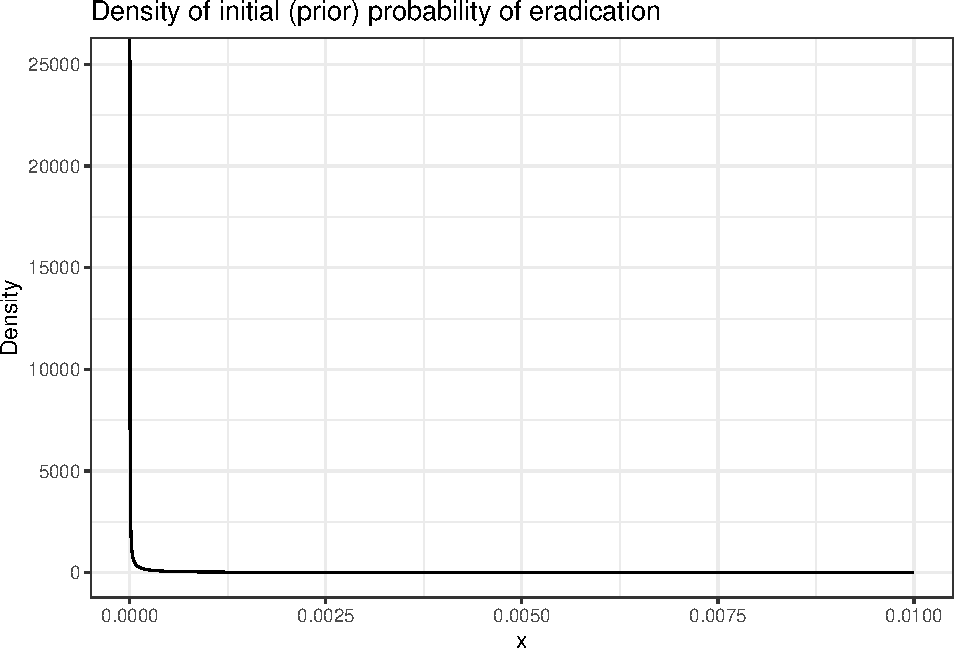
\includegraphics{_main_files/figure-latex/prior_init_size-3.pdf}
\caption{(\#fig:prior\_init\_size-3)Prior distribution of initial population size}
\end{figure}

As for the population sizes at later time points, I assume that growth is exponential at an uncertain rate. In particular, it is assumed that, for \(t \in \{2, \ldots, T\}\), \(N_t \mid N_{t-1}, R_t \sim \mathrm{Poisson}(N_{t-1} e^{R_t})\). Here, we can give any continuous distribution for \(R_t\). I have chosen the vaguely informative prior \(R_t \stackrel{\text{iid}} \sim \mathrm N(0, 20)\). The symmetry of this prior means that we are indifferent about whether the population is growing or declining.

The growth rate prior has been chosen to place most density below their estimated growth rate under optimal conditions. Medfly have been estimated to grow at 8\% per day, in optimal lab conditions (\citet{papadopoulos2002}). Under an exponential growth model this is 56\% per week. This can be taken as an extremely pessimistic upper bound on the growth rate. In real cases, flies may fail to establish due to food scarcity and unsustainability of population size. This is due to predation and other environmental pressures.

In real cases, it will be desirable to attempt to estimate \(R_t\) from data. In particular, it is known that fruit fly population growth rates are highly dependent on temperature. Therefore, it would be wise to estimate and draw values of \(R_t\) conditional on weather measurements. Choosing an empirically realistic distribution for \(R_t\) is likely to improve the efficiency of inference from the survey record.

\hypertarget{locations}{%
\subsection{Locations}\label{locations}}

\hypertarget{population-location}{%
\subsubsection{Population location}\label{population-location}}

\begin{itemize}
\tightlist
\item
  Overview
\item
  Technical details
\item
  Priors
\end{itemize}

For the distribution of the centre of the population, I have chosen a normal prior, centred at the origin (where the first fly was found). For details about this, see the appendix.

I first discuss the option of setting a uniform prior. Setting an uninformative prior is fairly straightforward for this problem. In particular, we might assume that, beyond a certain distance from the outbreak centre (say, 1km) any existing population of Medfly is distinct from the population of interest. Therefore, we might set the prior distribution for the population location to be uniform on the surface of a disk with 1km radius around the outbreak centre.

Despite the fact that an uninformative prior is relatively straightforward to set, it is most likely not advisable in specific applications. It will typically be the case that prior information is available to the decision maker. In particular, fruit flies are heavily dependent on the availability of suitable fruit trees for survival and reproduction. Therefore, someone with local area knowledge will be able to determine the most likely locations for an existing population. Also, the supplementary zone is not chosen arbitrarily. The choice of supplementary zone will typically reflect the beliefs of the decision maker about the location of the fly population.

When prior information exists, setting the prior distribution to be uninformative may cause us to underestimate the likelihood of observing captures in the supplementary surveillance zone. The overall effect will be to inflate \(\Pr(N_T = 0 \mid \mathbf y = \mathbf 0_T)\).

\hypertarget{individual-fly-dispersals}{%
\subsubsection{Individual fly dispersals}\label{individual-fly-dispersals}}

\begin{itemize}
\tightlist
\item
  Overview
\item
  Technical details
\item
  Priors
\end{itemize}

In release-recapture experiments, it is often the case that flies are released from a single point in the trapping grid (\citet{lg2004}, \citet{wong1982}). In the simplest model of detection, we might assume that this happens in the real world. In that case, the distance between each trap and each fly would just be the distance between that trap and the population. In other words, flies would all be clustered at a single point. However, this may not be reasonable in practice. Instead, it may be more reasonable to assume that flies are dispersed around a central point.

To incorporate dispersion of flies, I assume the following. Let \(L\) denote the central point of the population, as above. Then, let \(D_{i, t}\) denote the location of fly \(i\) at time \(t\), relative to the population centroid \(L\). For simplicity, it is assumed that \(D_{i, t}\) is independent of \(D_{i', t'}\), for any \((i', t') \neq (i, t)\). Thus, our belief is essentially that flies are shuffled around at each time point, so that a fly's location at \(t-1\) tells us nothing about its location at \(t\) (except through the information both reveal about \(L\)). This simply means that we do not track the locations of flies across time -- i.e., whether a fly lives across time periods, or instead dies and is replaced, are equivalent scenarios under this model.

The normal distribution is chosen for two reasons. Firstly, it is conceptually simple and intuitive to parameterise. Secondly, for mean zero normal random variables, distances to the origin have a known distribution. For example, let \[\mathbf X = (X_1, \ldots, X_p)^\top \sim \mathbf N_p(0, \sigma^2 I),\] where \(I\) is the \(p \times p\) identity matrix. Then the length of \(\mathbf X\), \(\lVert \mathbf X \rVert^{1/2} \sim \mathrm{Gamma}(??????)\) \citet{unfinished} (see appendix). This allows us to compare and calibrate the distribution against experimental results (see appendix). This, in turn, makes elicitation of priors simpler and more intuitive.

\hypertarget{the-detection-model}{%
\subsection{The detection model}\label{the-detection-model}}

\begin{itemize}
\tightlist
\item
  Overview
\item
  Technical details
\item
  Priors
\end{itemize}

\hypertarget{overview-1}{%
\subsubsection{Overview}\label{overview-1}}

The second key assumption is that we can estimate the probability of capturing a randomly selected fly from data. This is difficult in the case of Medfly. For fruit flies, capture probability is typically estimated from data taken from release-recapture studies. In these studies, the researcher obtains a large collection of sterilised specimens, and releases them at a single point in space. Then, the

These experimental data can be useful when the trapping setup is similar to the setup we want to draw inference about. However, this will often not be the case. For example, studies vary in the number and type of traps used (SEE NOTE). Further, we may wish to infer eradication of pest populations in trapping systems that are unlike those in studies. For example, after an outbreak has occurred, and eradication measures have been stopped, it is common to set up supplementary trapping units to intensify monitoring and increase the likelihood of detecting flies, conditional on their presence in the area. (\citet{supp_traps}).

The 16 extra traps are included because they increase the probability of detecting flies. Because they increase the likelihood of detections, they have a stronger effect on the posterior distribution.

\hypertarget{technical-details-1}{%
\subsubsection{Technical details}\label{technical-details-1}}

I assume that surveillance events occur at regular time intervals \(t \in \{1, \cdots, T\}\). The probability that a fly \(i\) is caught in trap \(k\) at time \(t\) is given by \(p_{i, k, t} = p(d_{i, k, t})\) where \(d\) is the distance between fly \(i\) and trap \(k\) at time \(t\), and \(p(\cdot)\) gives us the probability of capture as a function of distance.

\begin{itemize}
\tightlist
\item
  No interference.
\end{itemize}

\hypertarget{priors}{%
\subsubsection{Priors}\label{priors}}

I assume that the probability of capture is given by
\[
p(d) = \max(0.0073d^{-1.37}, 1),
\]
for \(d > 0\).

The results of release recapture studies are highly variable, and gaining access to data may be difficult for older studies. In this case, it may be desirable to incorporate uncertainty about the probability function. This could be done by definining a random. I do not explore this any further here, as this model exposition is intended for the purposes of illustration only.

\hypertarget{the-trapping-arrangement}{%
\subsubsection{The trapping arrangement}\label{the-trapping-arrangement}}

\begin{itemize}
\tightlist
\item
  Show plot of the trapping grid.
\item
  Note that the number of traps is assumed fixed as it would be in a real scenario.
\item
  Note that the trap locations would be known in a real analysis.
\end{itemize}

\hypertarget{computing-the-posterior-distribution}{%
\section{Computing the posterior distribution}\label{computing-the-posterior-distribution}}

In this section, I discuss the problem of computing the posterior distribution, given a survey record. Above, I stated that the model could be defined flexibly. Without restrictions on the form of the growth and detection models, the posterior may be analytically intractable. In other words, we will not be able to write out the posterior density or mass as a function of the data and prior distributions. Such situations are common in the Bayesian framework, because of the tendency for the posterior density or mass to depend, implicitly or explicitly, on analytically intractable integrals.

So far, we have talked about situations when sampling is required for inference. Further problems arise when the model is \emph{agent-based}. In other words, when we include uncertainty about individual-level features in the model. In this case, the detection probability is random, even when the location and population size is known. In other words, the probability of detecting at least one individual is a function of the number of individuals, and also their individual (random) properties. This is a situation in which ``the number of things you do not know is one of the things you do not know'' (Richardson and Green, 1997).

A simple rejection algorithm is used to draw samples from the posterior distribution.

\hypertarget{abc-models}{%
\subsection{ABC models}\label{abc-models}}

ABC methods, as exemplified by Caley's model, are a promising approach. Here, I will give a brief description of the family of sampling algorithms known collectively as Approximate Bayesian Computation (ABC). In its simplest form, ABC is a form of rejection sampling.

\hypertarget{motivation-for-abc}{%
\subsection{Motivation for ABC}\label{motivation-for-abc}}

There are two reasons for sampling with ABC. Firstly, the likelihood may be unattractive to work with due to its complexity. Secondly, when our model incorporates uncertainty about the individual members of a population, whose size is itself uncertain, standard sampling techniques do not work.

Two things should be noted before moving on. Firstly, the reader may note that the justification given for ABC is unusual. ABC is relatively recent technique for sampling in cases where traditional sampling techniques fail. Standard techniques for MCMC, such as Metropolis-Hastings and Gibbs sampling, assume that the likelihood function is known and can be easily computed. This may not be the case if, for example, computing the likelihood requires us to integrate out a latent variable, but the likelihood is not integrable with respect to that variable.

Secondly, the reader may note that there exist other methods for sampling from the posterior.

Here, I have used EBC for intuitiveness, ease of implementation, and the fact that it is relatively efficient for this problem. However, other methods exist that may be worth exploring, for analogous problems where the rejection rate of ABC is higher. There are at least two known methods for sampling from the posterior when the dimension of the parameter space is uncertain. These are the reversible jump MCMC sample (\citet{green1995}) and the generalised Gibbs sampler (\citet{keith2015}). These may be worth exploring for problems where the rejection rate is high for EBC.

Interestingly, the standard justifications for and against ABC do not apply to the case under consideration. Firstly, the standard justification for ABC is that it allows for inference when the likelihood function is ``intractable'' - i.e., unknown, uncomputable or otherwise difficult to work with. However, for the current model, the likelihood is known, and relatively simple to write out.

On the other hand, the standard drawback for ABC is that it ensures that we can typically only draw from the posterior approximately. Under standard conditions, we must define a criteria for similarity between simulated and observed data. This is typically done by specifying a summary statistic \(S(\mathbb y)\), and a similarity measure \(\rho(S(\mathbb y), S(\mathbb y'))\) defined over the space spanning our data \(\mathbb y\). We reject a sample if we observe \(\rho(\mathbb y_{\text{observed}}, \mathbb y_{\text{simulated}} ) > \epsilon_0\), where \(\epsilon_0\).

\hypertarget{results}{%
\section{Results}\label{results}}

\begin{itemize}
\item
  How long did sampling take?
\item
  What was the rejection rate?
\item
  The fly free period is 12 weeks or 28 days and one generation, whichever is longer (\citet{meats2005}). In summer, a Medfly generation takes 28-34 days (\citet{dpirdwa}). Therefore, the period I look at is over 12 weeks. However, this may be different based on the period that the manager is interested in.
\end{itemize}

\hypertarget{probability-of-extinction-after-12-weeks}{%
\subsection{Probability of extinction after 12 weeks}\label{probability-of-extinction-after-12-weeks}}

\hypertarget{discussion}{%
\section{Discussion}\label{discussion}}

Here I discuss limitations and objections.

\hypertarget{drawbacks}{%
\subsection{Drawbacks}\label{drawbacks}}

\begin{itemize}
\tightlist
\item
  We do not get a posterior distribution over the probability of eradication.
\end{itemize}

\hypertarget{objections}{%
\subsection{Objections}\label{objections}}

\hypertarget{bayesian-models-are-too-subjective}{%
\subsubsection{Bayesian models are too subjective}\label{bayesian-models-are-too-subjective}}

\hypertarget{bayesian-models-are-too-sensitive-to-priors}{%
\subsubsection{Bayesian models are too sensitive to priors}\label{bayesian-models-are-too-sensitive-to-priors}}

\begin{itemize}
\tightlist
\item
  Defence in Caley 2015
\end{itemize}

% Trigger ToC creation in LaTeX
\renewcommand{\baselinestretch}{1}\normalsize

\hypertarget{appendices}{%
\chapter{Appendices}\label{appendices}}

\hypertarget{appendix-1-proof-of-abc-procedure}{%
\section{Appendix 1: Proof of ABC procedure}\label{appendix-1-proof-of-abc-procedure}}

Here, I give a proof that the simple ABC rejection algorithm yields independent draws from the posterior distribution. Recall that the algorithm works by drawing samples of \(\theta\) from the prior distribution with density \(\pi (\theta)\). Then, for each draw of \(\theta\), we draw a data vector \(y_{\text {sim}}\) from the likelihood \(l(\theta \mid y_{\text{sim}})\). Finally, we keep the sample if we observe that \(y_{\text{sim}} = y_{\text{obs}}\) (where \(y_{\text{obs}}\) is the data vector we actually observed) and reject it otherwise. Then, the draws that we keep have distribution \(f_{\text{ABC}}(\theta) = \pi(\theta) \cdot l(\theta \mid y_{\text{obs}})\), since our draws from the prior and likelihood are independent.

\footnote{Credit is due to (this StackExchange post){[}\url{https://stats.stackexchange.com/questions/380076/proof-of-approximate-exact-bayesian-computation}.{]}.}

\hypertarget{appendix-2-full-model-statement}{%
\section{Appendix 2: Full model statement}\label{appendix-2-full-model-statement}}

\[
\renewcommand{\baselinestretch}{1}\normalsize
\begin{aligned}
&\textbf{Population size} \\
&\text{Initial no. of flies:} && N_1 \mid \lambda \sim \mathrm{Pois}(\lambda) \text{, where} \\
&&& \lambda \sim \mathrm{Exponential}(1/20) \\
& \text{Rate of increase:}~ && R_t \sim \mathrm{Normal}(\mu_t, \sigma^2_t), & t \in \{2, \ldots, T \} \\
& \text{No. of flies:}~ && N_t := \mathrm{round} \{ N_{t-1} \exp(R_t) \}    & t \in \{2, \ldots, T\} \\
\\
&\textbf{Fly locations} \\
& \text{Popn. loc.:}~ && L^{(U)} \sim \mathrm{Uniform}^2(200, 600) \\
&&& L^{(N)} \sim \mathrm{Normal}^2(0, \sigma) \\
&&& L := L^{(U)} + L^{(N)} \\
& \text{Fly dispersals:}~ && D_{i,t} \sim \mathrm{Normal}(0, 20) & i \in \{1, \ldots, N_t\}, \\
  &&&& t \in \{1, \ldots, T\}\\
& \text{Fly locations:}~ && L_{i,t}^\text{fly} := L + D_{i,t} & i \in \{1, \ldots, N_t\}, \\
  &&&& t \in \{1, \ldots, T\}\\
\\
&\textbf{Detection model} \\
& \text{No. traps:}~ && K \in \mathbb N_+ \\
& \text{Trap locations:}~ && L_k^\text{trap} & k \in \{1, \ldots, K\} \\
& \text{Dist. btw. fly } i \text{ and trap } k \text{ at time } t \text{:} && \delta_{i,k,t} := \lVert L_k^\text{trap} - L_{i,t}^\text{fly} \rVert & i \in \{1, \ldots, N_t\}, \\
  &&&& k \in \{1, \ldots, K\}, \\
  &&&& t \in \{1, \ldots, T\}\\
& \text{Individ. cap. prob.:} && p_{i, t} = 1 - \prod_{k=1}^K (1 - p(\delta_{i,k,t})), & i \in \{1, \ldots, N_t\}, \\
  &&&& k \in \{1, \ldots, K\}, \\
  &&&& t \in \{1, \ldots, T\}\\
&  && \mathbf p_t := [p_{i,t}]_{i=1}^{N_t}  & t \in \{1, \ldots, T\} \\
&\text{No. of captures:}~ && y_t \mid \theta \sim \text{Poisson-binomial}(N_t, \mathbf p_t), & t \in \{1, \ldots, T\} \\
  &&& \mathbf y := [y_t]_{t=1}^T
\end{aligned}
\renewcommand{\baselinestretch}{1}\normalsize
\]

\hypertarget{appendix-3-population-location-prior}{%
\chapter{Appendix 3: Population location prior}\label{appendix-3-population-location-prior}}

To update on detection location when the first fly is detected at a trap (say trap k) we can use a trick. The trick is to model the probability of the first detection being at trap k as the probability that a fly is detected at k in one period conditional on exactly one fly total being detected in that period. The benefit of this model is that it does not depend on how many weeks it took to get the first detection (which would require information about how long flies have been around before the first detection). See appendix for more details.

A mathematical trick can be used to derive a prior in some cases. Suppose we have \(K\) traps indexed by \(k \in \{1, \ldots, L\}\). Suppose also that we have a prior distribution over the population size \(N\), given by \(N \sim \mathrm{Poisson} (\lambda)\), with \(\lambda \sim \mathrm{Exponential(1/20)}\). Here we assume no change in population size over time. Now, we suppose that each trap \(k\) is ``competing'' to catch the first trap each week. We suppose that the trap at the centre of the grid was the first to catch a fly, and we want to use this information. Define the random variable
\[
C_k = \begin{cases}1 & \text{a fly is caught in trap } k \text{ before any other trap} \\ 0 & \text{otherwise}. \end{cases}
\]

Under these assumptions, \(L \mid C_k = 1\) is the distribution of \(L\), given that a fly was caught in trap \(k\) before any other trap.

Whether or not we can analytically derive the posterior density depends on the probability of capture function \(p(x)\). In the case we consider here, the function cannot be integrated, and so I resort to sampling. Under the above assumptions, the posterior resembles the convolution of a normal and a uniform distribution (see figure). See appendix for more details.

\hypertarget{appendix-1-proof-of-abc-procedure-1}{%
\chapter{Appendix 1: Proof of ABC procedure}\label{appendix-1-proof-of-abc-procedure-1}}

Here, I give a proof that the simple ABC rejection algorithm yields independent draws from the posterior distribution. Recall that the algorithm works by drawing samples of \(\theta\) from the prior distribution with density \(\pi (\theta)\). Then, for each draw of \(\theta\), we draw a data vector \(y_{\text {sim}}\) from the likelihood \(l(\theta \mid y_{\text{sim}})\). Finally, we keep the sample if we observe that \(y_{\text{sim}} = y_{\text{obs}}\) (where \(y_{\text{obs}}\) is the data vector we actually observed) and reject it otherwise. Then, the draws that we keep have distribution \(f_{\text{ABC}}(\theta) = \pi(\theta) \cdot l(\theta \mid y_{\text{obs}})\), since our draws from the prior and likelihood are independent.

\footnote{Credit is due to (this StackExchange post){[}\url{https://stats.stackexchange.com/questions/380076/proof-of-approximate-exact-bayesian-computation}.{]}.}

\hypertarget{appendix-3-population-location-prior-1}{%
\chapter{Appendix 3: Population location prior}\label{appendix-3-population-location-prior-1}}

To update on detection location when the first fly is detected at a trap (say trap k) we can use a trick. The trick is to model the probability of the first detection being at trap k as the probability that a fly is detected at k in one period conditional on exactly one fly total being detected in that period. The benefit of this model is that it does not depend on how many weeks it took to get the first detection (which would require information about how long flies have been around before the first detection). See appendix for more details.

A mathematical trick can be used to derive a prior in some cases. Suppose we have \(K\) traps indexed by \(k \in \{1, \ldots, L\}\). Suppose also that we have a prior distribution over the population size \(N\), given by \(N \sim \mathrm{Poisson} (\lambda)\), with \(\lambda \sim \mathrm{Exponential(1/20)}\). Here we assume no change in population size over time. Now, we suppose that each trap \(k\) is ``competing'' to catch the first trap each week. We suppose that the trap at the centre of the grid was the first to catch a fly, and we want to use this information. Define the random variable
\[
C_k = \begin{cases}1 & \text{a fly is caught in trap } k \text{ before any other trap} \\ 0 & \text{otherwise}. \end{cases}
\]

Under these assumptions, \(L \mid C_k = 1\) is the distribution of \(L\), given that a fly was caught in trap \(k\) before any other trap.

Whether or not we can analytically derive the posterior density depends on the probability of capture function \(p(x)\). In the case we consider here, the function cannot be integrated, and so I resort to sampling. Under the above assumptions, the posterior resembles the convolution of a normal and a uniform distribution (see figure). See appendix for more details.

  \bibliography{book.bib,packages.bib}

\end{document}
